\chapter{Action Ragionally}
\section{Agents and environments}
\textbf{Agents} include humans, robots, softbots, thermostats, etc.
The agent function maps from percept histories to actions: 
\[f: \mathcal{P}^* \rightarrow \mathcal{A}\]
The agent program runs on the physical architecture to produce $f$.
\subsubsection{Example: Vacuum-cleaner world}
\begin{figure}[H]
    \centering
    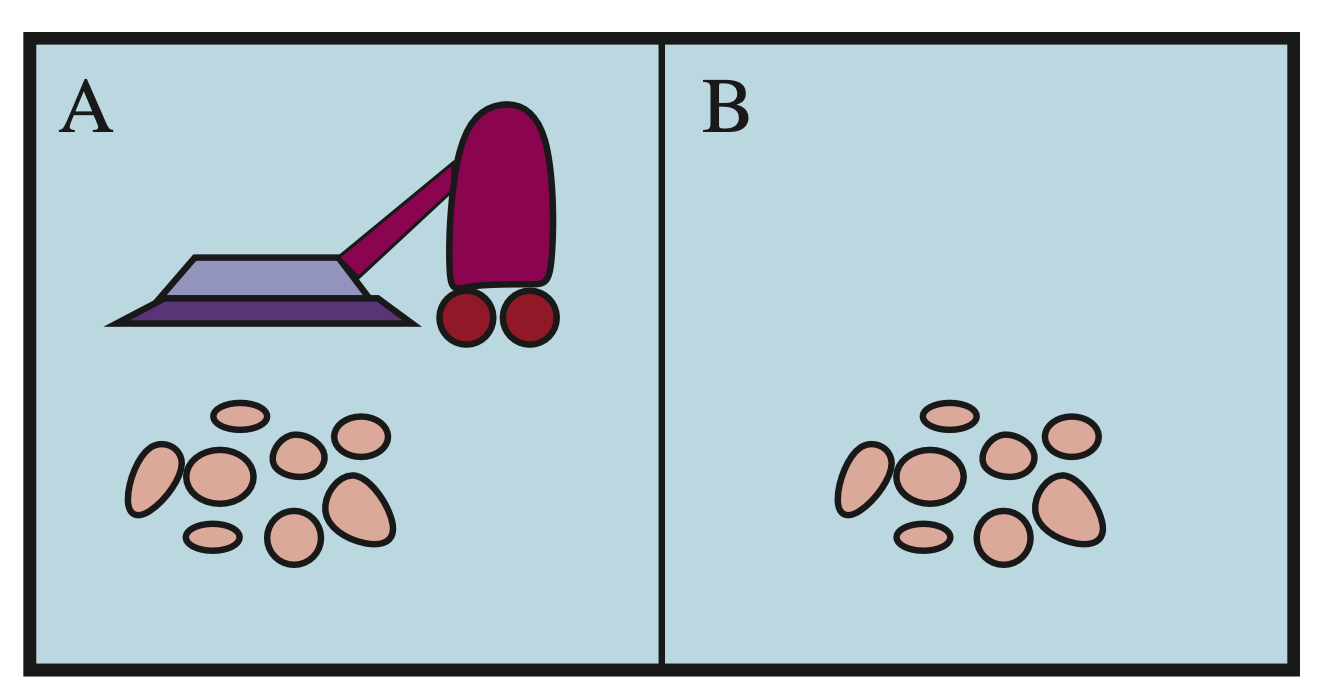
\includegraphics[width=0.5\textwidth]{img/vacuum-cleaner.png}
    \caption{A vacuum-cleaner world with just two locations. Each location can be either clean or dirty. 
    The agent perceives the location and the status of the location (clean/dirty). 
    The agent can move left, right, suck, or do nothing.}
    \label{fig:vacuum_cleaner_world}
\end{figure}
\begin{tabular}[H]{|cc|}
    \hline
    \textbf{Percept sequence} & \textbf{Action} \\
    \hline
    \verb|[A, Clean]| & Right \\
    \verb|[A, Dirty]| & Suck \\
    \verb|[B, Clean]| & Left \\
    \verb|[B, Dirty]| & Suck \\
    \verb|[A, Clean], [A, Clean]| & Right \\
    \verb|[A, Clean], [A, Dirty]| & Suck \\
    \vdots & \vdots \\
    \verb|[A, Clean], [A, Clean], [A, Clean]| & Right \\
    \verb|[A, Clean], [A, Clean], [A, Dirty]| & Suck \\
    \vdots & \vdots \\
    \hline
\end{tabular} 

What is the right function $f$?
\begin{tcolorbox}[title = {Agent Programs vs Agent functions}]
    \textbf{Agent program} is the implementation of the agent function.
    If an agent has $|\mathcal{P}|$ possible perceptions, the entries
    in the table after $T$ time steps will be 
    $
    \sum_{t=1}^{T} | \mathcal{P}|^t
    $
\end{tcolorbox}
The artificial intelligent goal is to design small agent programs that 
can represent large agent functions.
A possible agent program for the vacuum-cleaner world is:
\begin{lstlisting}[language=Python, basicstyle=\small]
    function Reflex-Vacuum-Agent([location, status]) returns an action
        if status == Dirty then return Suck
        else if location == A then return Right
        else if location == B then return Left
\end{lstlisting}
\section{Rationality}
Fixed \textbf{performance measure} evaluates the environment sequences
\begin{itemize}
    \item one point per square cleaned up in the timer $T$?
    \item one point per clean square per time step, minus one point per move?
    \item penalizefor $> k$ dirt squares?
\end{itemize}
A ragional agent chooses whichever action maximizes the expected 
value of the performance measure given the percept sequence to date.
but we have to know that \textbf{rational} $\not =$ \textbf{omniscient}. Percepts may not
supply all relevant information.
We have also the problem of \textbf{rational} $\not =$ \textbf{clairvoyant}.
Actions outcomes may not be as expected.
And then \textbf{Hence, rational} $\not =$ \textbf{successful}.

Rational means exploration, learning, and autonomy.
\section{PEAS (Performance measure, Environment, Actuators, Sensors)}
To design a rational agent, we must specify the task environment 
in which it is to operate.
Lets consider the example of a taxi driver.
\begin{itemize}
    \item \textbf{Performance measure}: safe, fast, legal, comfortable trip, maximize profits
    \item \textbf{Environment}: roads, other traffic, pedestrians, customers, weather, etc.
    \item \textbf{Actuators}: steering wheel, accelerator, brake, signal, horn, display, etc.
    \item \textbf{Sensors}: cameras, sonar, speedometer, GPS, odometer, engine sensors, etc.
\end{itemize}
\section{Environment types}
The environments types are:
\begin{itemize}
    \item \textbf{Fully observable} vs \textbf{partially observable}
    \item \textbf{Deterministic} vs \textbf{stochastic}
    \item \textbf{Episodic} vs \textbf{sequential}
    \item \textbf{Static} vs \textbf{dynamic}
    \item \textbf{Discrete} vs \textbf{continuous}
    \item \textbf{Single-agent} vs \textbf{multi-agent}
\end{itemize}
The \textbf{environment type largely determines the agent design}.
The real world is \textbf{partially observable}, \textbf{stochastic}, \textbf{sequential}, \textbf{dynamic}, \textbf{continuous}, and \textbf{multi-agent}.
\section{Agent types}
We can define an agent:
\[
  agent = architecture \,+\, program  
\]
The general Skeleton for a program is:
\begin{itemize}
    \item input: current perception
    \item output: next action
\end{itemize}
Four basic types in order of increasing generality:
\begin{itemize}
    \item \textbf{Simple reflex agents}
    \item \textbf{Model-based reflex agents}
    \item \textbf{Goal-based agents}
    \item \textbf{Utility-based agents}
\end{itemize}
All these can be turned into \textbf{learning agents}.
\subsection{Simple reflex agents}
\begin{figure}[H]
    \centering
    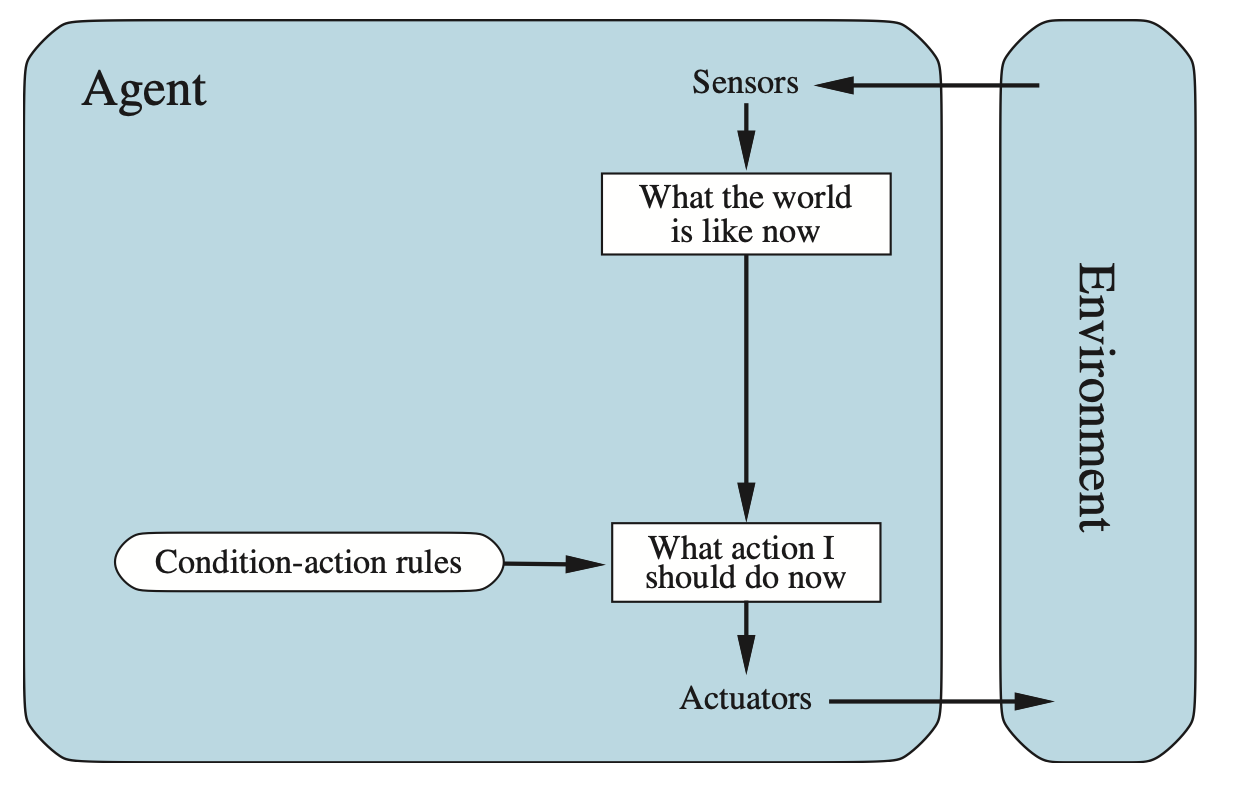
\includegraphics[width=0.5\textwidth]{img/reflex-agents.png}
    \caption{Simple reflex agent}
    \label{fig:simple_reflex_agent}
\end{figure}
\begin{lstlisting}[language=Python, basicstyle=\small]
    function Reflex-Vacuum-Agent([location, status]) returns an action
        if status == Dirty then return Suck
        else if location == A then return Right
        else if location == B then return Left
\end{lstlisting}
\subsection{Reflex agents with state}
\begin{figure}[H]
    \centering
    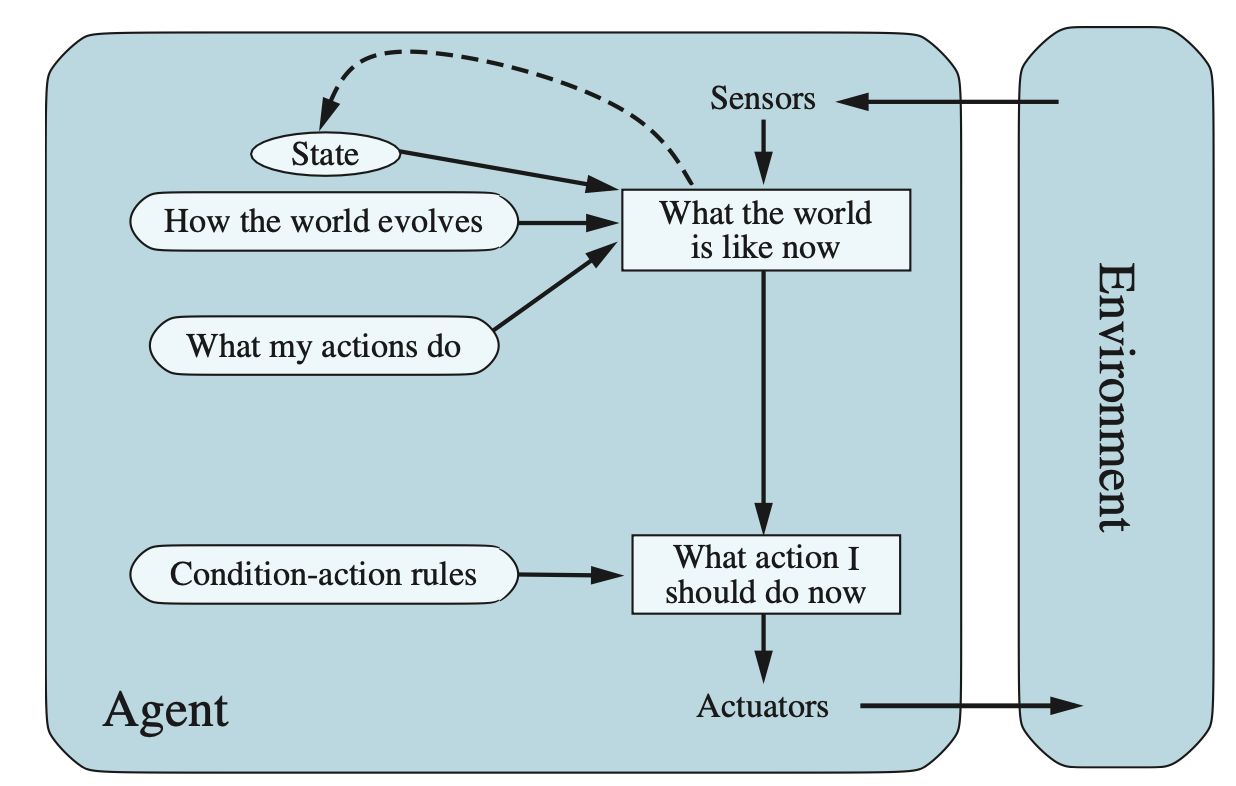
\includegraphics[width=0.5\textwidth]{img/reflex-agents-with-state.png}
    \caption{Reflex agent with state}
    \label{fig:reflex_agent_with_state}
\end{figure}
\begin{lstlisting}[language=Python, basicstyle=\small]
    function Reflex-Vacuum-Agent([location, status]) returns an action
        static: current-location, current-status,
        current-action = none,
        next-action = none
        
        current-location = Update-State(current-location, current-action)
            if status = Dirty then next-action = Suck
            else if current-locondition = A then next-action = Right
            else if current-condition = B then next-action = Left
            current-action = next-action
            return current-action
\end{lstlisting}
\subsection{Goal-based agents}
\begin{figure}[H]
    \centering
    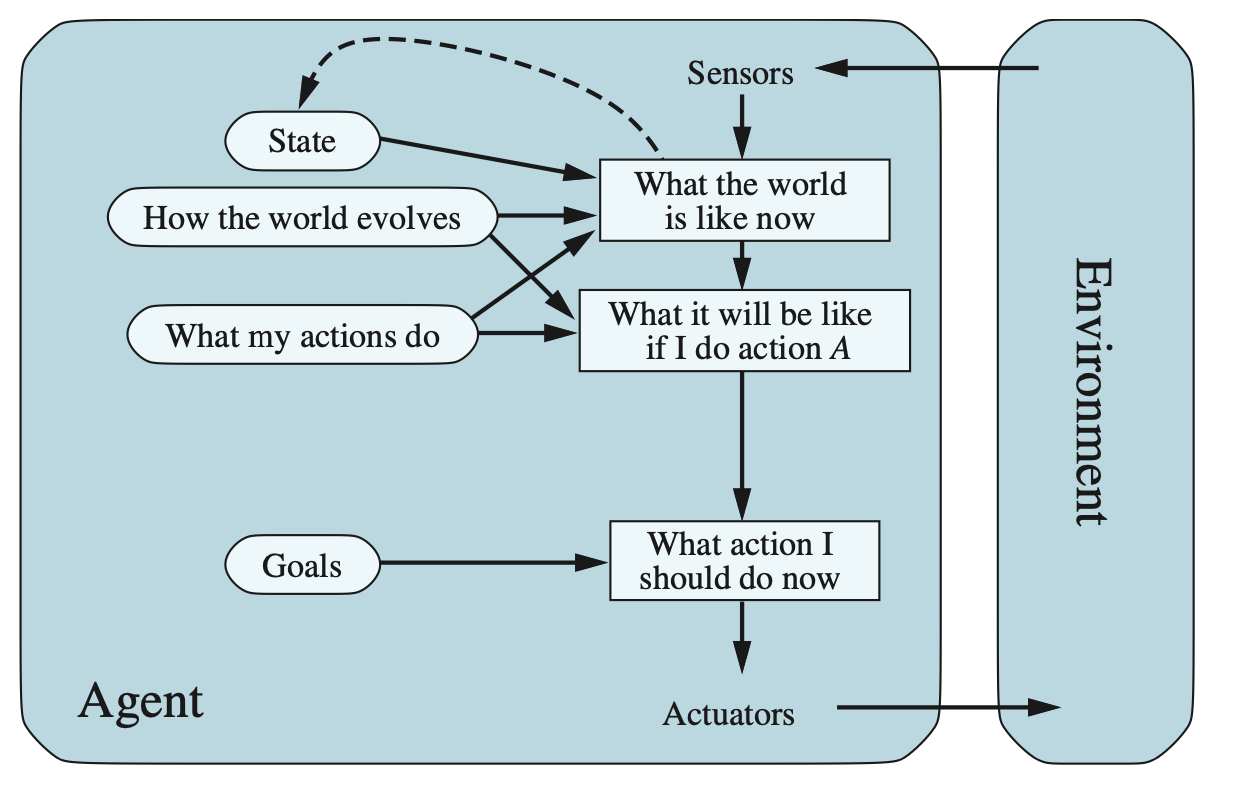
\includegraphics[width=0.5\textwidth]{img/goal-based-agents.png}
    \caption{Goal-based agent}
    \label{fig:goal-based-agents}
\end{figure}
\subsection{Utility-based agents}
\begin{figure}[H]
    \centering
    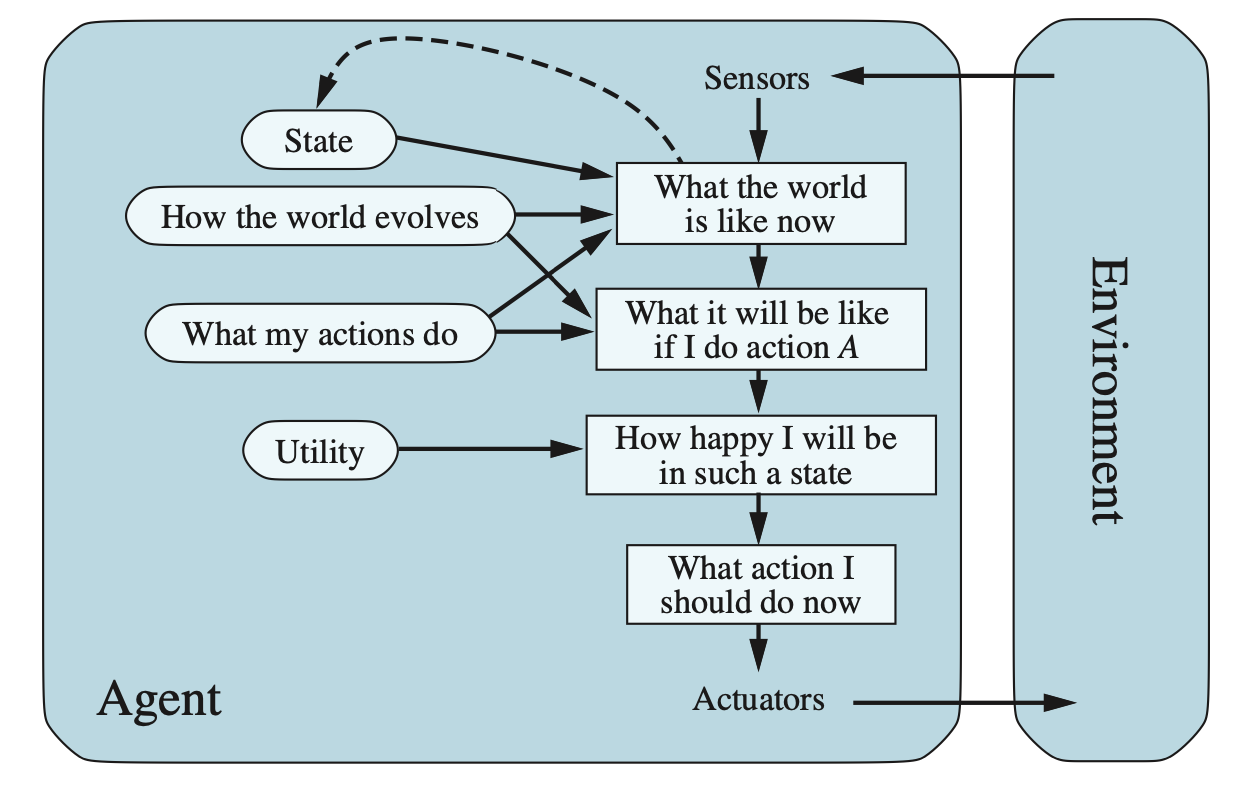
\includegraphics[width=0.5\textwidth]{img/utility-based-agents.png}
    \caption{Utility-based agent}
    \label{fig:utility-based-agents}
\end{figure}
\subsection{Learning agents}
\begin{figure}[H]
    \centering
    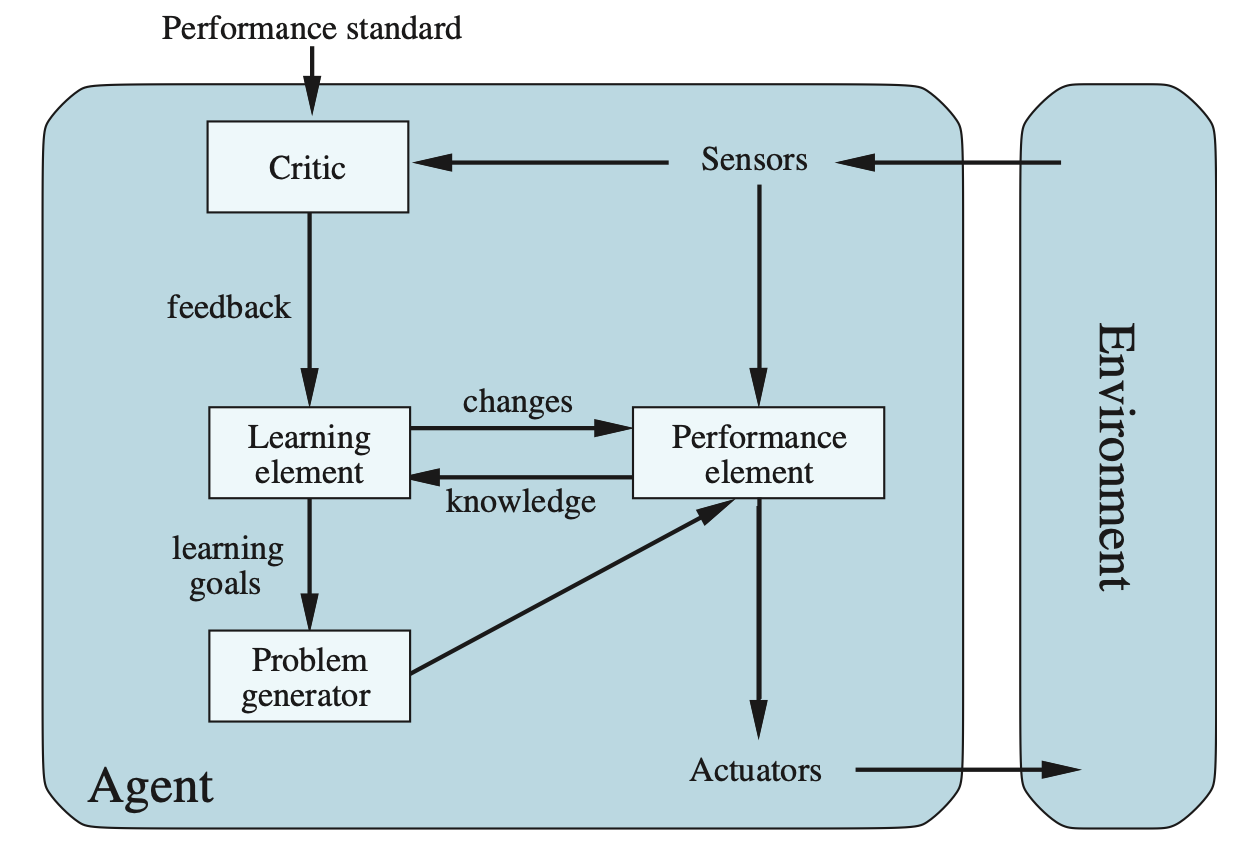
\includegraphics[width=0.5\textwidth]{img/learning-agents.png}
    \caption{Learning agent}
    \label{fig:learning-agents}
\end{figure}
\subsection{Summary}
Agents interact with environments through actuators and
sensors. The agent function describes what the agent
does in all circumstances. The performance measure
evaluates the environment sequence. A perfectly
rational agent maximizes expected performance. Agent
programs implement (\textit{some}) agent functions. \verb|PEAS|
descriptions define task environments. Environments
are categorized along several dimensions:
\begin{itemize}[label=--, left=1em]
    \item Observable?
    \item Deterministic?
    \item Episodic?
    \item Static?
    \item Discrete?
    \item Single-agent?
\end{itemize}

Several basic agent architectures exist:
\begin{itemize}[label=--, left=1em]
    \item Reflex
    \item Reflex with state
    \item Goal-based
    \item Utility-based
\end{itemize}
